\documentclass{beamer}
%\usepackage{fontspec} 
\usepackage{soul}
\usepackage{tikz}
\usepackage{pgfplots}
\newcommand{\barplot}[4]{%
  \begin{tikzpicture}
    \begin{axis}[
	xlabel={#1},  
	ylabel={#2}, 
	axis lines*=left, 
        width  = \textwidth,
	height = .3\textheight,
    	nodes near coords, 
	xtick=data,
	x tick label style={},  
	ymin=0,
	symbolic x coords={#3},
	]
	\addplot+[ybar,lsRichGreen!80!black,fill=lsRichGreen] plot coordinates {
	    #4
	}; 
    \end{axis} 
  \end{tikzpicture} 
}

\useoutertheme{lsp}

\usepackage{lsptitle}

\def\two@digits#1{\ifnum#1<10 0\fi\number#1}
\def\mytoday{\two@digits{\number\day}.\two@digits{\number\month}.\number\year}


\usepackage{xspace,multicol}
\newcommand{\latex}{\LaTeX\xspace}
\usepackage{tikz}


\newcounter{lastpagemainpart}
\footnotesep0pt
\renewcommand{\footnoterule}{}
\usefootnotetemplate{
  \noindent
  \insertfootnotemark\insertfootnotetext}

\let\beamerfn=\footnote
\renewcommand{\footnote}[1]{%
\let\oldfnsize=\footnotesize%
\let\footnotesize=\tiny%
\beamerfn<\thebeamerpauses->{#1}%
\let\footnotesize=\oldfnsize}


\date{20.10.2026}

\usepackage{eurosym}  
 
\renewcommand{\centerline}[1]{\hfill#1\hfill\hfill\mbox{}}

\title{Scholar-led publishing and Diamond Open Access:  \mbox{the funding and business model of}
\mbox{Language Science Press}}
\author[LangSci]{Alena Witzlack-Makarevich (U of Bremen)}

\begin{document}
\lspbeamertitle

\section{Introduction}

\frame{
    \frametitle{Language Science Press}
    \begin{itemize}
        \item LSP has been active since 2014
        \item Publishes monographs and edited volumes in linguistics 
        \item Born from the insight that:
        \begin{itemize}
            \item Community-based publishing of scientific literature \\(in linguistics) will be more cost-efficient than publishing by commercial publishers.
            \item New technologies and collaborative work methods mean that many traditional tasks performed by publishers are no longer needed or can be provided at a fraction of the cost.
        \end{itemize}
    \end{itemize}
}

\frame{
\frametitle{The beginning}
\begin{itemize}
 \item First contact: 2012
 \item Active since 2014
 \begin{itemize}
   \item 2014--2016 FU Berlin (DFG seed funding)
   \item 2016--2018 HU Berlin
   \item 2019-- non-profit limited liability company (gemeinnützige UG)
 \end{itemize}
\end{itemize} 
}

\frame{
\frametitle{The team}
\begin{itemize}
\item currently directed by Stefan Müller (FU Berlin), \\Oliver Czulo (U of Leipzig, Translatologie gGmbH), \\and Alena Witzlack-Makarevich (U of Bremen)
\item press coordinator: Sebastian Nordhoff
\item a small team of linguists and programmers
\item in the early stages, there was also a business manager 
\end{itemize}
}

\frame{
\frametitle{The principles of LSP}

\begin{enumerate}
    \item \textbf{Diamond/Platinum Open Access:} No fees for authors or readers worldwide, low-cost print-on-demand copies, and open publication processes.
    \item \textbf{Quality:} Mandatory peer review and high publication standards.
    \item \textbf{Specialization:} Specialized series ensure quality according to subdisciplinary standards.
    \item \textbf{Decentralized Organization:} Autonomous series editors manage submissions and quality.
    \item \textbf{Community:} Researchers contribute through authorship, reviewing, and proofreading.
    \item \textbf{Automation:} Standardized workflows and tools to streamline production and reduce costs.
    \item \textbf{Lean Publishing:} OA publishing avoids legacy activities such as warehousing, royalties, and paywalls.
\end{enumerate}
}

\section{2025}

\frame{
\frametitle{12 years later}
    \begin{columns}[c]
        \begin{column}{0.57\textwidth}
\begin{itemize}
\item as of today, 376 books published 
\item all books Diamond/Platinum Open Access
\item current goal: 33 books/year 
\item 39 series including
    \begin{itemize}
    \item Studies in Diversity Linguistics: 33 books
    \item Translation and Multilingual Natural Language Processing: 27 books
    \item Textbooks in Language Sciences: 22 books
    \item Open Germanic Linguistics: \\17 books
    \end{itemize}
\end{itemize}
\end{column}

        \begin{column}{0.43\textwidth}
            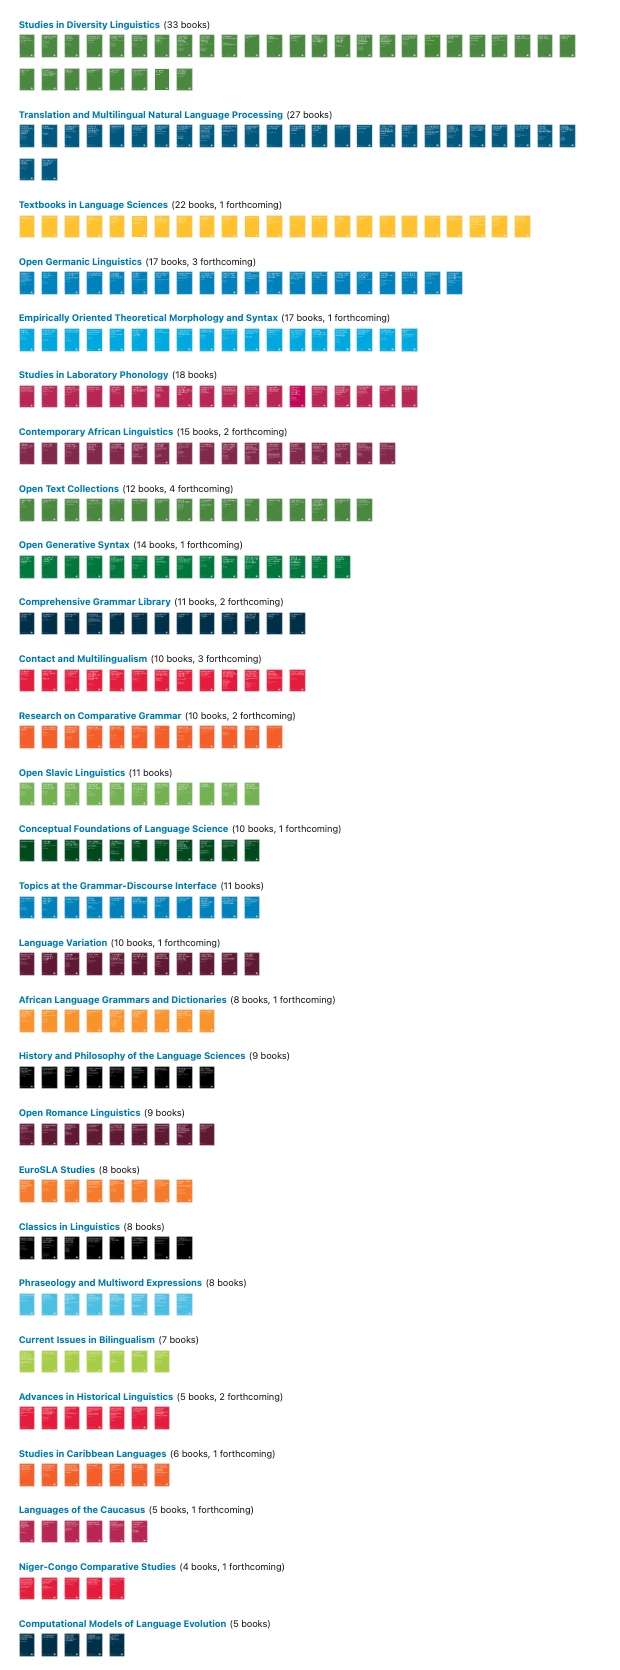
\includegraphics[
                width=\linewidth,
                height=0.95\textheight,
                keepaspectratio
            ]{series.png}
        \end{column}

    \end{columns}
}

\frame{
    \frametitle{Achievements 2025}
    \begin{columns}[c]
        \begin{column}{0.63\textwidth}
            \textbf{2025 Publications}
            \begin{itemize}
   \item 39 books were published
   \item 124 works were proposed to LSP
   \item compare to 95 in 2024 \\and 109 in 2023
   \item submission to decision:\\75 days (median)
\item submission to publication: 339 days %(median)
\item the acceptance rate (incl.\,desk rejections): 57.88\% over all series
%\item the acceptance rate for submissions where the manuscript had gone into peer review: 92.10\%
\item pdfs downloaded 656,276 times
\item most downloaded: \textit{Arabic and contact-induced change} (23,566)

            \end{itemize}
        \end{column}
        \begin{column}{0.37\textwidth}
            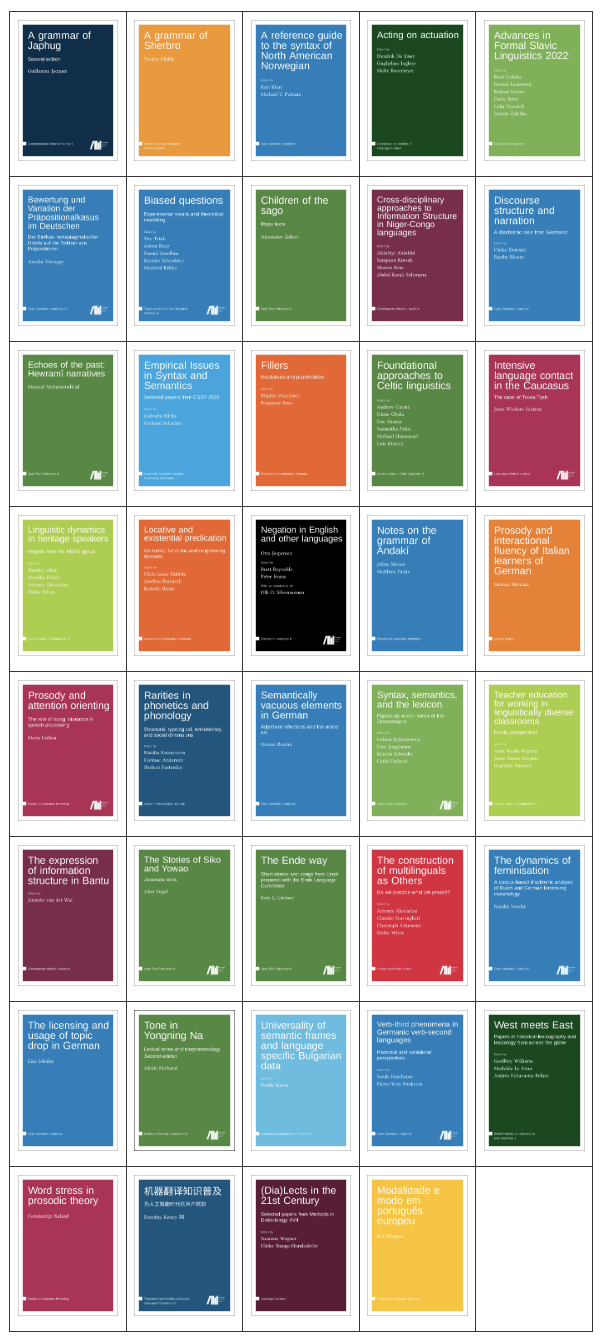
\includegraphics[
                width=\linewidth,
                height=0.9\textheight,
                keepaspectratio
            ]{volumes2025.png}
        \end{column}

    \end{columns}
}

%\frame{ 
% 	\frametitle{Workflow} 	
 %   \begin{center}
 %       \includegraphics[
%            width=0.95\textwidth,
%            height=0.9\textheight,
%            keepaspectratio
%        ]{workflow.png}
%    \end{center}
% }

\section{Workflow}
\frame{
\frametitle{Workflow}
\begin{itemize}
\item initial submission of papers
\item reviewing \& acceptance/rejection of papers
\item revised papers
\item conversion to \textbf{LaTeX} (with \textbf{Overleaf}): editors' task, but assistance is given. LSP does a rough conversion, postprocessing is done by  volume editors; the closer the initial papers follow the \textbf{templates} and the stylesheet, the less time-consuming it is.)
\item proofreading (\textbf{Paperhive}) \& indexing
\item incorporation of proofreaders’ comments
\item final typesetting
\item approval by volume editor and signing of contract
\item approval by series editor and by press directors
\item preparation of print-on-demand
\item publication as pdf and print (+various online venues)
\item announcement
\end{itemize}
}

\section{Community}

\frame{
\frametitle{The community}
    \begin{columns}[c]
        \begin{column}{0.57\textwidth}
\begin{itemize}
\item over 1900 supporters
\item an international Advisory Board of 13 renowned scholars
\item over 1400 linguists have published a book or a chapter
\item over 652 community proofreader, 314 in 2025 (see Hall of Fame)
\end{itemize}
\end{column}

        \begin{column}{0.43\textwidth}
            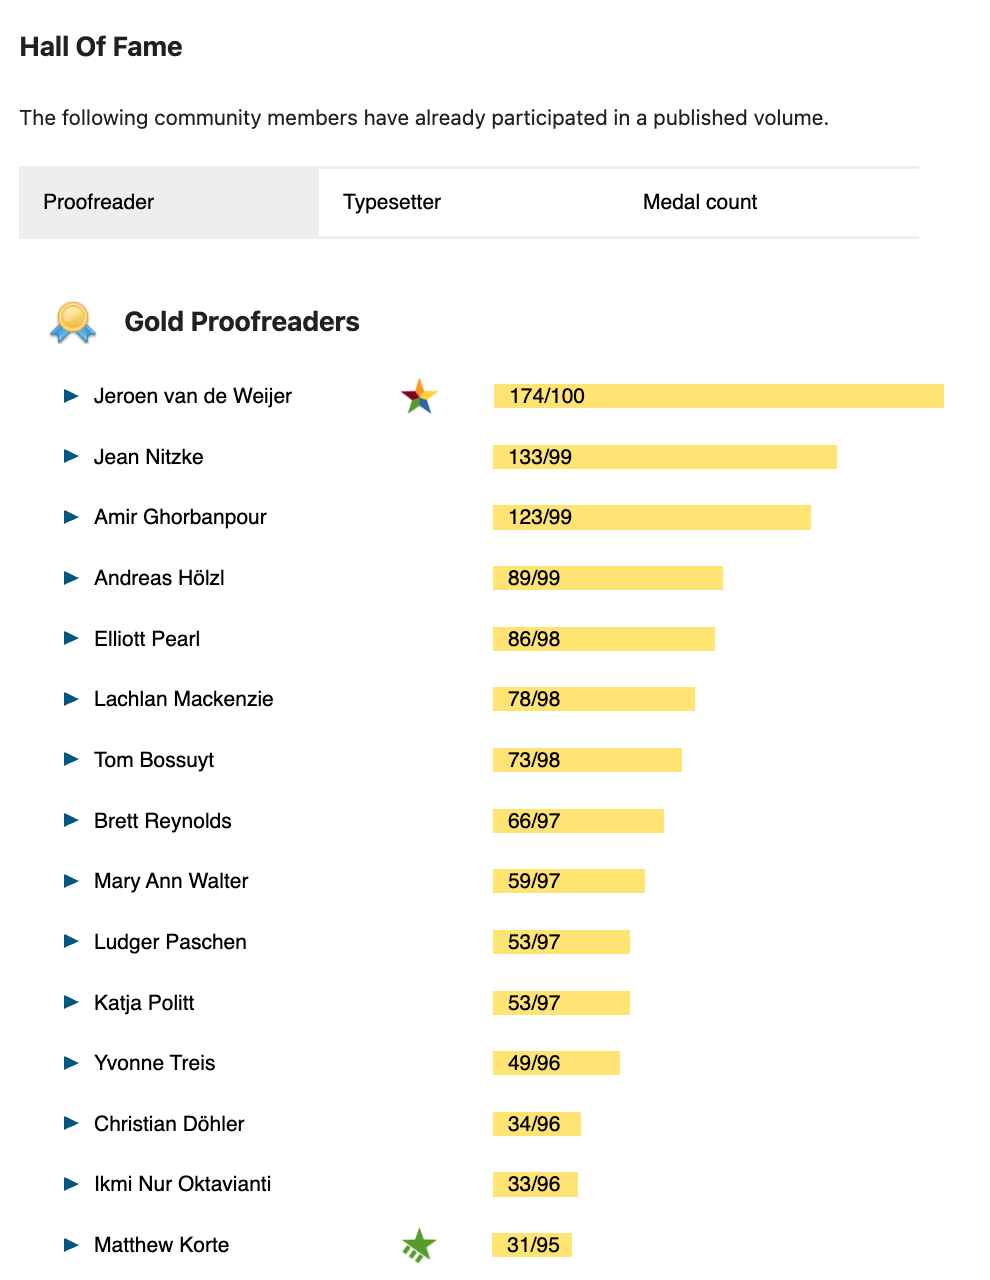
\includegraphics[
                width=\linewidth,
                height=0.95\textheight,
                keepaspectratio
            ]{hallOfFame.png}
        \end{column}
    \end{columns}
}


\frame{
\frametitle{A typical community member}

    \begin{columns}[c]
        \begin{column}{0.57\textwidth}
            \begin{itemize}
                \item Edited one volume (2018, over 43,000 downloads)
                \item Published one monograph (2021, over 8,900 downloads)
                \item Authored three articles in edited volumes
                \item Reviewed one monograph and a few articles
                \item Proofread chapters in 18 volumes
                \item About to start a new series: Open Dictionaries Collection
                \item Since 2023: member of the Advisory Board 
            \end{itemize}
        \end{column}

        \begin{column}{0.43\textwidth}
            \centering
            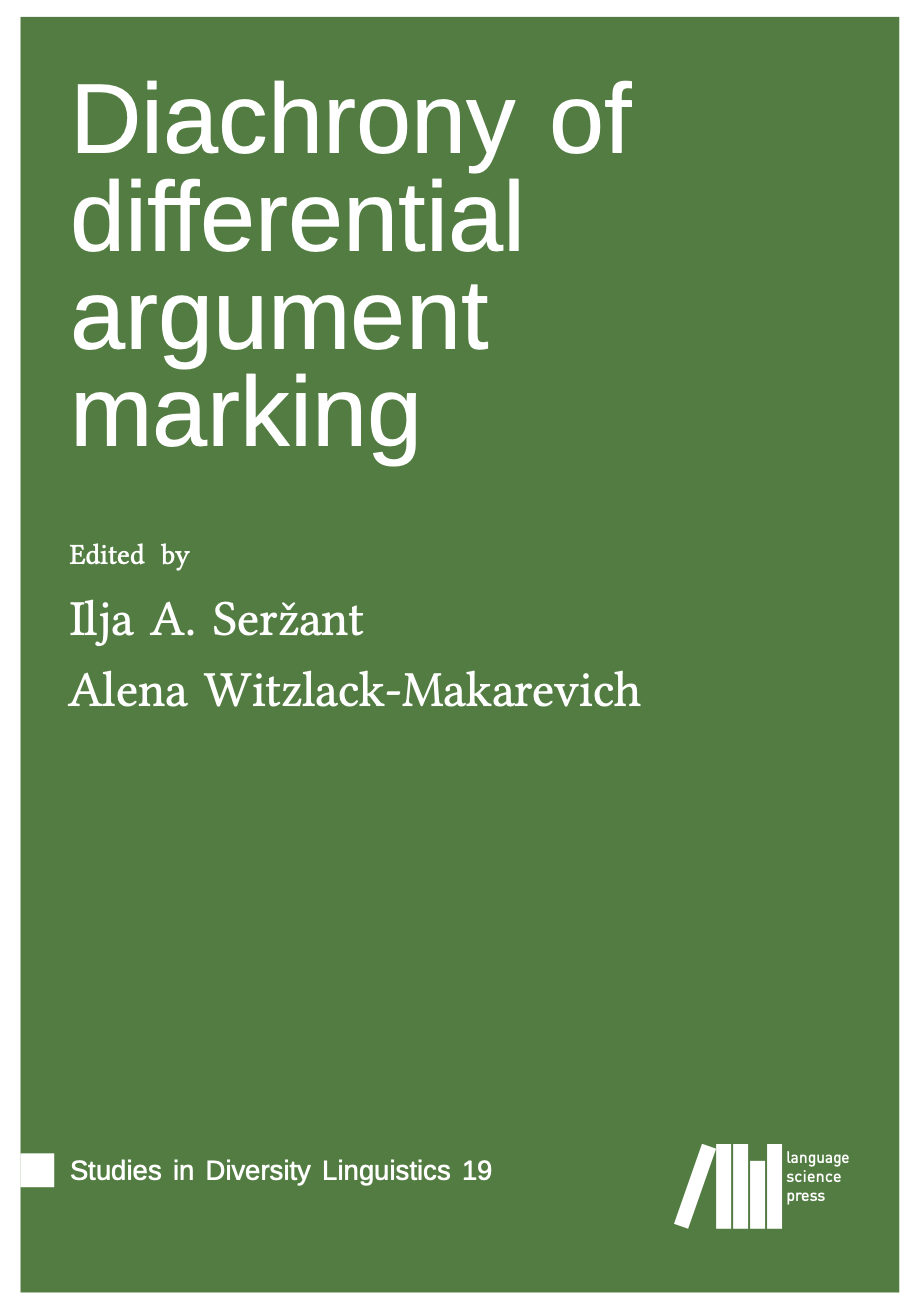
\includegraphics[
                width=0.85\linewidth,
                height=0.45\textheight,
                keepaspectratio
            ]{DOM.png}

            \vspace{0.3cm}

            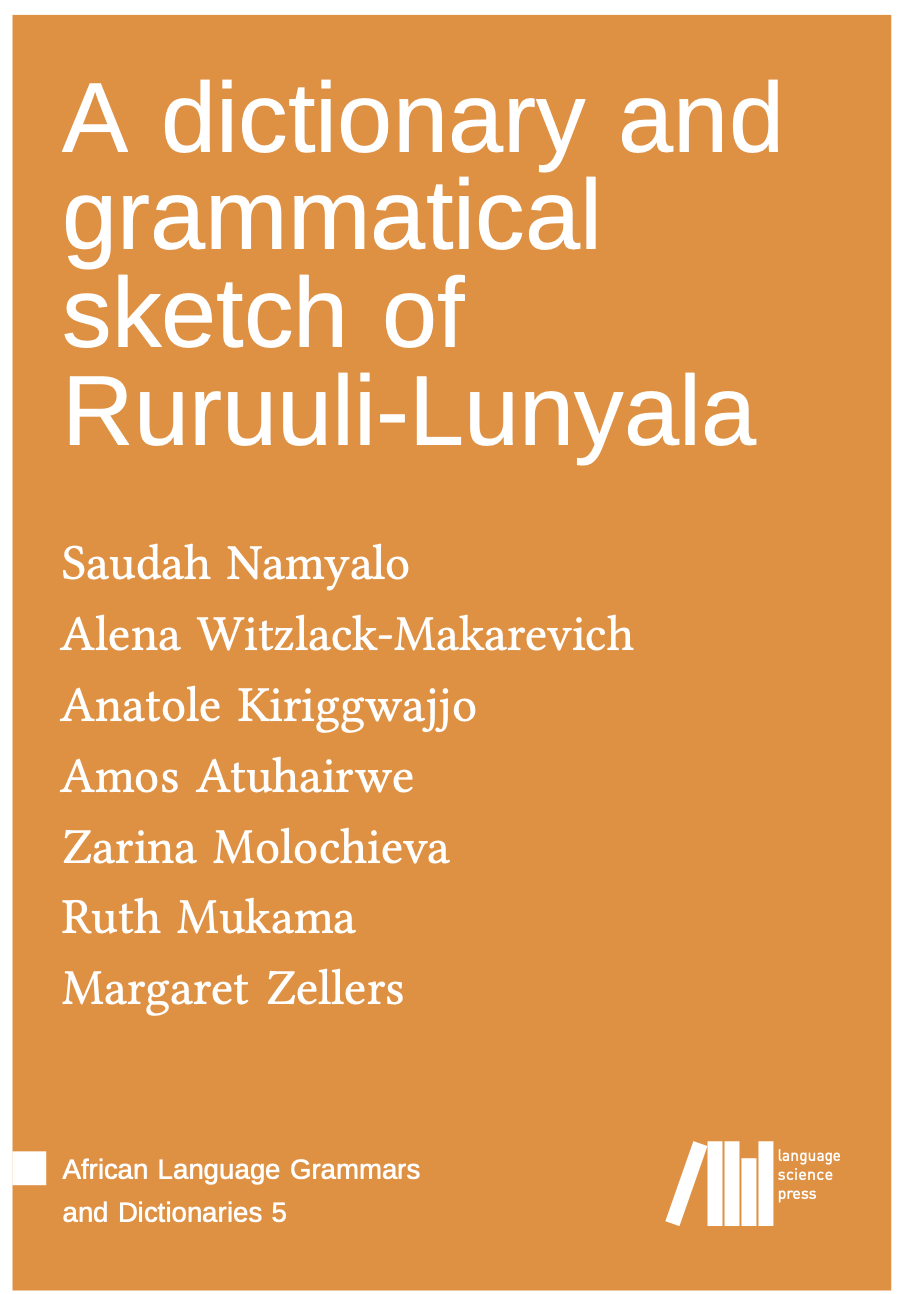
\includegraphics[
                width=0.85\linewidth,
                height=0.45\textheight,
                keepaspectratio
            ]{Ruuli.png}
        \end{column}
    \end{columns}
}

\section{Business model}
\frame{
\frametitle{Business model}
 \textit{Replicable strategies for book publications supplemented with empirical data}\\
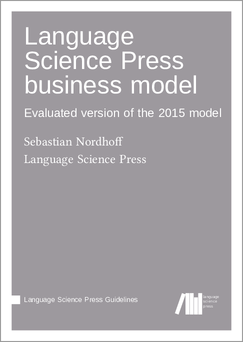
\includegraphics[width=.35\textwidth]{businessmodel.png}\hfill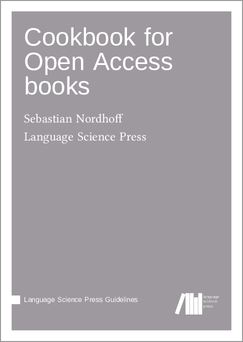
\includegraphics[width=.35\textwidth]{cookbook.png}\hfill
~

\url{langsci-press.org/opendata}
}

\frame{
\frametitle{Business model}
\begin{itemize}
 \item Publishing does not come for free
    \begin{itemize}
    \item Obvious costs: ink and paper, computer storage, 
    \item Not-so-obvious costs: the time needed to set up a book for print-on-demand or the creation of user manuals and screencasts
    \end{itemize}

\item These costs have to be counterbalanced by revenue
\item Traditionally, publishers recoup their costs via the margin of their book sales
\item In an open access paradigm with a smaller print run, this is less straightforward
\end{itemize}
}

\frame{
\frametitle{Finances 2025}
\begin{itemize}
\item Expenditures of 143,870.24 € (+2,417.81 €)
 \item A revenue of 153,223.04 € (+ 7,522.91 €) 
\item What's the break down?
\end{itemize}
}

\frame{

\frametitle{Expenses 2025}

%    \begin{itemize}
%   \item Personnel:  113,829.25 €, \\7 employees of three different nationalities
%\item Service providers: 7,417.49 €
%\item Rent: 11,066.43 €
%\item Travel: 4,613.35 €
%\item Book copies: 4,730.22 €
%    \end{itemize}

 %   \begin{center}
        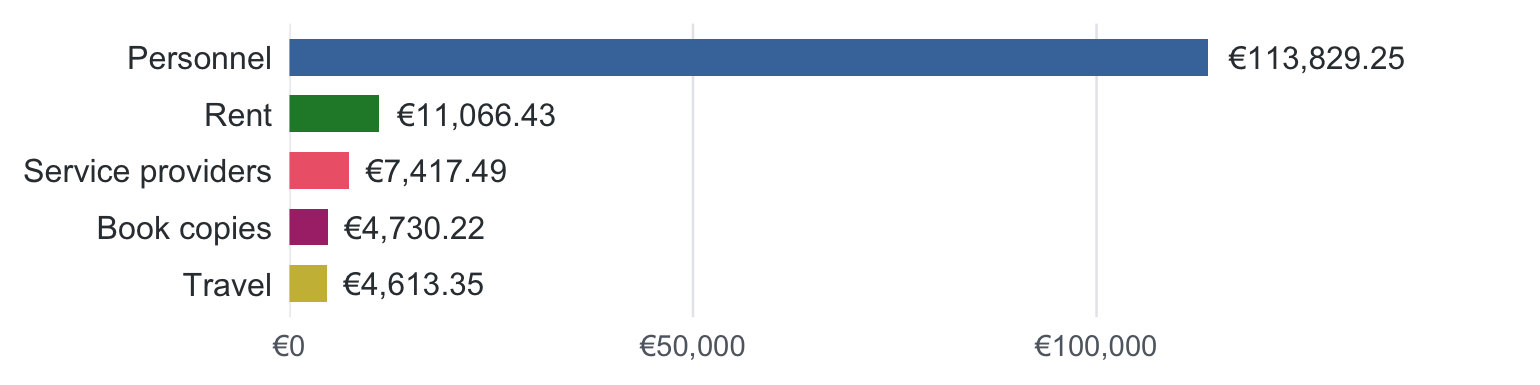
\includegraphics[
            width=0.9\textwidth,
            height=0.9\textheight,
            keepaspectratio
        ]{2025expenses.png}
%    \end{center}
}


\frame{
\frametitle{What does a book cost?}

\begin{itemize}
   \item Costs for producing a fully open access book (CC-BY):\\around 4,000 EUR (3,700 in 2025)
  \item this is the global sum we need per book: the cost is met by all participating institutions and individuals together
  \item compare this to the quotes of 10,000 EUR (de Gruyter) or 18,500 EUR (Brill)
  \item possible only thanks to all the free support we receive from the community!
\end{itemize}

}
\frame{
    \frametitle{Revenue 2025}

%    \begin{itemize}
 %       \item Institutional memberships \\via Knowledge Unlatched: 138,645 €
 %       \item Book sales: 8,679.85 €
%        \item Donations, PBCs: 579.76 €
%    \end{itemize}

    \begin{center}
        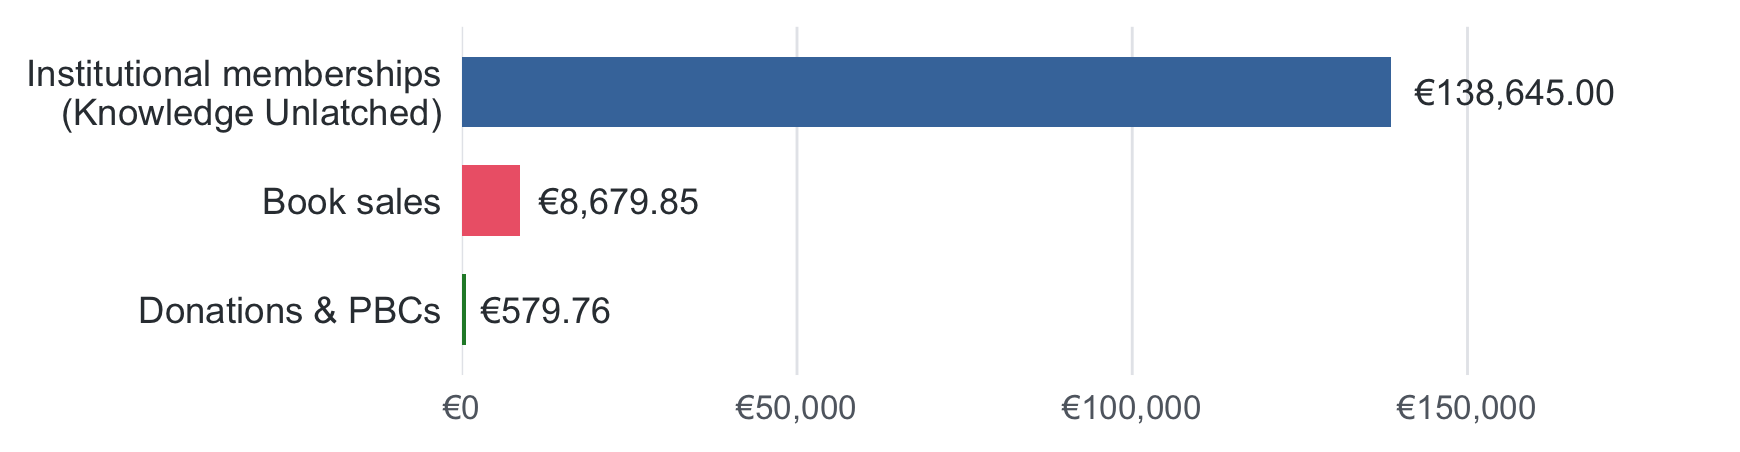
\includegraphics[
            width=0.95\textwidth,
            height=0.9\textheight,
            keepaspectratio
        ]{2025revenue.png}
    \end{center}
}

\frame{
    \frametitle{Institutional memberships}

    \begin{itemize}
       \item 2023-2026: funding from 112 institutions
            \begin{itemize}
        \item Adam Mickiewicz University Poznan
        \item Central Library of Zürich
        \item Institute for Croatian Language and Linguistics
        \item Johns Hopkins University
        \item State and University Library Bremen
        \item …
   \end{itemize}
 \item Facilitated via Knowledge Unlatched
\end{itemize}

  \begin{center}
        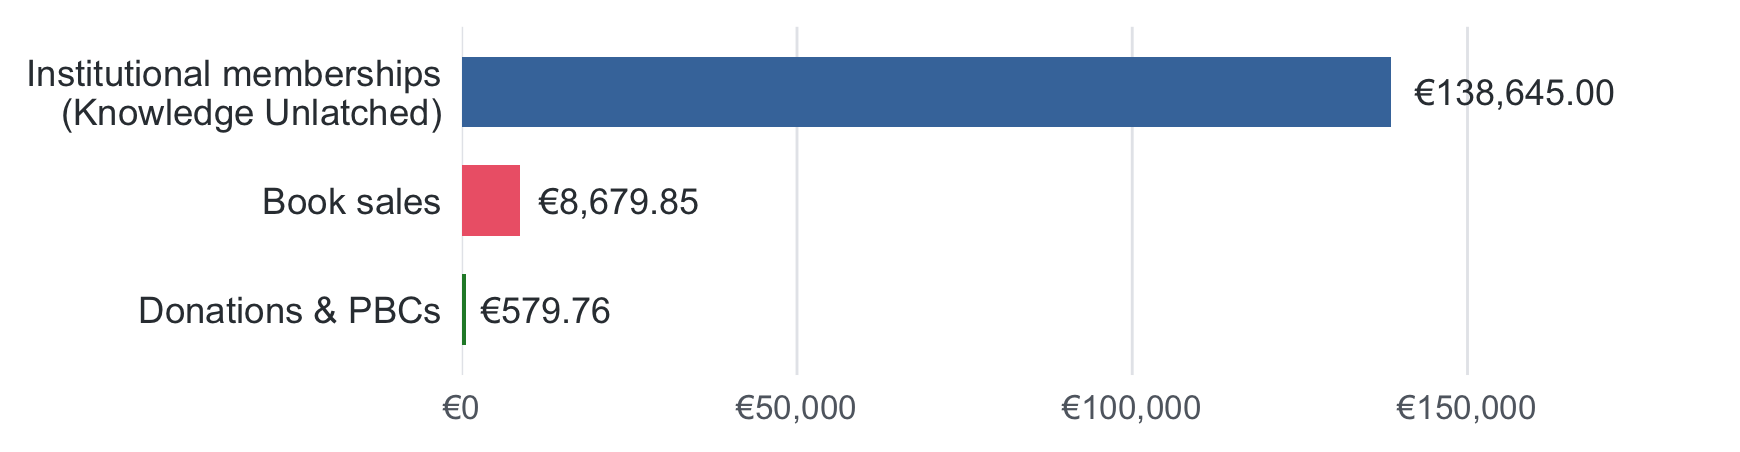
\includegraphics[
            width=0.95\textwidth,
            height=0.9\textheight,
            keepaspectratio
       ]{2025revenue.png}
  \end{center}
}

\frame{
    \frametitle{Knowledge Unlatched}

    \begin{itemize}
\item Knowledge Unlatched (KU) is an OA service provider
\item Established in 2012 as a British not-for-profit Community Interest Company (CIC)
\item In 2016 the legal structure changed to Knowledge Unlatched GmbH, registered as a for-profit in Berlin, Germany
\item In 2021, acquired by Wiley
\item In 2025, the journal publisher Annual Reviews signed an agreement with Wiley to acquire Knowledge Unlatched (KU), returning it to nonprofit management
\item Currently 15\% commission
   \end{itemize}
}

\frame{
    \frametitle{Knowledge Unlatched}

    \begin{itemize}
\item Libraries contribute: Libraries worldwide pledge funds to support selected books or collections.
\item Publication costs are shared: Contributions from multiple institutions help cover the costs of making books openly accessible.
\item Publishers provide OA editions: Supported titles are made available online under appropriate OA licenses.
\item Readers benefit: Researchers, students, and the public can access and download books without subscription or purchase barriers.
\item Scope: Humanities and Social Sciences

   \end{itemize}
}

\frame{
    \frametitle{Institutional memberships}
    \begin{itemize}
       \item For the period 2027-2029, 40 institutions have already pledged support
        \item More institutions are needed to join the pledge
        \item Many thanks in advance!

   \end{itemize}
}
%\setcounter{framenumber}{\thelastpagemainpart}
\end{document}
